\documentclass[tikz,border=6pt]{standalone}
\begin{document}
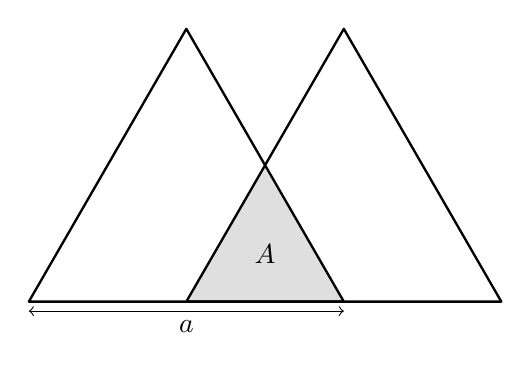
\begin{tikzpicture}[line cap=round,line join=round]
\fill[gray!25] (2,0)--(4,0)--(3,{sqrt(3)})--cycle;
\draw[line width=.85pt] (0,0)--(4,0)--(2,{2*sqrt(3)})--cycle;
\draw[line width=.85pt] (2,0)--(6,0)--(4,{2*sqrt(3)})--cycle;
\node at (3,.6) {$A$};
\node[below] at (2,-.12) {$a$};
\draw[thin,<->] (0,-.12)--(4,-.12);
\end{tikzpicture}
\end{document}
